%----------------------------------------------------------------------------------------
%	PROGETTAZIONE
%----------------------------------------------------------------------------------------

\section{Progettazione}
Il processo di sviluppo adottato ha visto due fasi di progettazione ben distinte: il design architetturale e il design di dettaglio.\\

\subsection{Design Architetturale}

Dapprima il gruppo si è concentrato sul design architetturale, ovvero la definizione dell'architettura generale del sistema, delle sue componenti principali e delle relazioni tra di esse.\\
Ciò ha permesso di individuare fin da subito gli elementi più importanti del sistema e di definire le interfacce tra di essi, nonchè di scegliere le tecnologie più appropriate
per supportare il core del sistema.\\

Fin dalle prime fasi di analisi sono emersi due domini distinti ma connessi tra di loro:
\begin{itemize}
    \item \textbf{User Domain}: comprende tutti i componenti del sistema che concorrono a fornire un'interfaccia di accesso al sistema all'utente finale.
    \item \textbf{Charging Station Domain}: comprende tutti i componenti del sistema che concorrono a modellare il comportamento delle Charging Station e di monitornarne costantemente lo stato.
\end{itemize}

In seguito all'individuazione di questi domini, il gruppo ha individuato per ognuno di essi le componenti principali, che verranno di seguito discusse. \\

Per quanto riguarda lo User Domain:
\begin{itemize}
    \item \textbf{User App}: applicativo utilizzato dall'utente finale, costituisce l'interfaccia principale con il sistema, permettendo di visualizzare i dati e di interagire con esso.
    \item \textbf{Auth Server}: servizio che permette di registrare ed autenticare gli utenti permettendo loro di accedere al sistema. \\
    \item \textbf{User DB}: database che contiene le informazioni sugli utenti registrati al sistema.
\end{itemize}

La User App, all'avvio, richiederà all'utente di autenticarsi o registrarsi e genererà una richiesta HTTP da inviare all'Auth Server. Quest'ultimo interrogherà il database per verificare l'esistenza
dell'utente o per crearne uno nuovo. In seguito alla riuscita di queste operazioni, l'utente avrà accesso alla User App e potrà interagire con il sistema.\\

Per quanto riguarda il Charging Station Domain:
\begin{itemize}
    \item \textbf{Charging Station}: componente hardware che permette di ricaricare le batterie dei veicoli elettrici.
    \item \textbf{Charging Station Actor}: componente software che gestisce la Charging Station, permettendo di monitorare lo stato della stessa e di interagire con essa.
    \item \textbf{Charging Station Provider}: componente software che osserva lo stato delle Charging Station e ne fornisce un'interfaccia di accesso.
    \item \textbf{Charging Station Service}: sotto componente del Charging Station Provider, permette di esporre l'interfaccia del Charging Station Provider attraverso una API REST. \\
\end{itemize}

Siccome i dati relativi alle Charging Station sono conosciuti ed utilizzati dal Charging Station Actor, il gruppo ha deciso di non creare al momento un Database per memorizzarli, ma di utilizzare un modello a scambio di messaggi per effettuare
query direttamente sui Charging Station Actors.\\

I vari Charging Station Actors dunque gestiscono in maniera indipendente le Charging Station, e comunicano in maniera peer-to-peer con il Charging Station Provider, il quale può sia essere notificato
dai Charging Station Actors di eventuali cambiamenti di stato, sia interrogato dalla User App per ottenere informazioni sullo stato delle Charging Station attraverso l'API REST esposta dal Charging Station Service.\\

L'architettura complessiva del sistema è dunque riassunta nel seguente diagramma:

\begin{figure}[htbp]
    \centering
    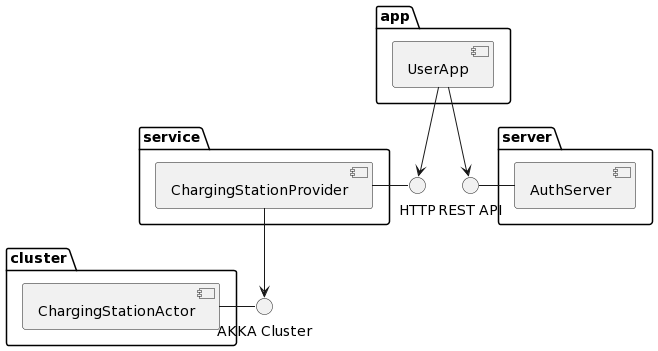
\includegraphics[width=\textwidth]{images/architecture.png}
    \caption{Diagramma dei Componenti per l'architettura del sistema}
    \label{fig:architecture}
\end{figure}

\subsubsection{Interazione tra le componenti del sistema}
Una volta individuate le componenti principali del sistema, il gruppo ha definito le interazioni tra di esse, in modo da poter definire le interfacce di comunicazione tra loro.\\
In seguito saranno riportate le interazioni tra le componenti del sistema, elencate per caso d'uso.\\

\paragraph{Signup di un utente}
L'utente inizia il processo di registrazione nell'applicazione. L'utente interagisce con l'applicazione utente e fornisce un nome utente, un indirizzo email e una password per registrarsi.

L'applicazione utente invia quindi una richiesta di registrazione al servizio di autenticazione. Questo, a sua volta, comunica con un database degli utenti.

Il servizio di autenticazione cerca nel database se l'indirizzo email fornito dall'utente è già presente. In caso negativo esso comunica all'applicazione utente che l'utente è stato registrato con successo, e l'applicazione utente restituisce una risposta positiva all'utente.

Tuttavia, se l'indirizzo email è già presente nel database, il servizio di autenticazione informa l'applicazione utente che l'indirizzo email è già in uso, e l'applicazione utente restituisce una risposta negativa all'utente.

In entrambi i casi, l'applicazione utente fornisce una risposta all'utente per comunicare l'esito della registrazione.

Questa interazione è riassunta nel seguente diagramma di sequenza:
\begin{figure}[htbp]
    \centering
    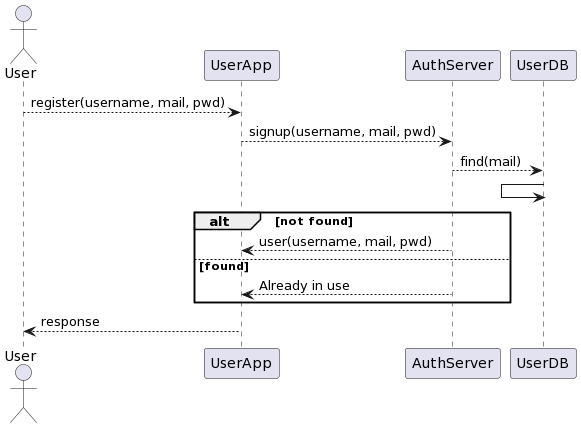
\includegraphics[width=\textwidth]{images/signup.png}
    \caption{Diagramma delle sequenze per la registrazione di un utente}
    \label{fig:signup}
\end{figure}

\paragraph{Login di un utente}
L'utente inizia il processo di accesso (login) nell'applicazione. L'utente interagisce con l'applicazione utente e fornisce il proprio indirizzo email e la password per effettuare l'accesso.

L'applicazione utente invia quindi una richiesta di accesso al Servizio di Autenticazione. Questo servizio comunica con un database degli utenti.

Il Servizio di Autenticazione cerca nel database le credenziali fornite dall'utente per verificare se corrispondono a un account registrato. Se le credenziali sono corrette (caso di successo), il Servizio di Autenticazione comunica all'applicazione utente che l'utente è stato autenticato con successo, e l'applicazione utente restituisce una risposta positiva all'utente.

Tuttavia, se le credenziali fornite non sono corrette (caso di fallimento), il Servizio di Autenticazione informa l'applicazione utente che l'indirizzo email o la password sono errati, e l'applicazione utente restituisce una risposta negativa all'utente.

In entrambi i casi, l'applicazione utente fornisce una risposta all'utente per comunicare l'esito del tentativo di accesso.\\

Questa interazione è riassunta nel seguente diagramma di sequenza:
\begin{figure}[htbp]
    \centering
    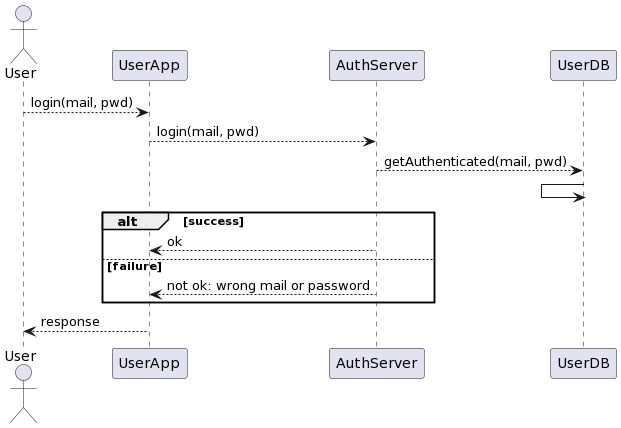
\includegraphics[width=\textwidth]{images/login.png}
    \caption{Diagramma delle sequenze per il login di un utente}
    \label{fig:login}
\end{figure}

\paragraph{Visualizzazione dello stato di una stazione di ricarica}
L'utente interagisce con l'applicazione utente e seleziona una stazione di ricarica.

L'applicazione utente invia quindi una richiesta per ottenere informazioni sulla stazione di ricarica selezionata al Charging Station Service. Questo a sua volta comunica con il Provider.

Il Provider cerca le informazioni sulla stazione di ricarica identificata dall'ID nella richiesta. Se la stazione di ricarica viene trovata (caso di successo), il Provider comunica al Service che ha avuto successo, e restituisce le informazioni trovate.

Tuttavia, in caso di fallimento, il Provider comunica che non è riuscito a trovare la stazione di ricarica specificata.

In base all'esito, il Charging Station Service comunica all'applicazione utente la risposta, che verrà quindi visualizzata all'utente dall'applicazione utente.

Questa interazione è riassunta nel seguente diagramma di sequenza:

\begin{figure}[htbp]
    \centering
    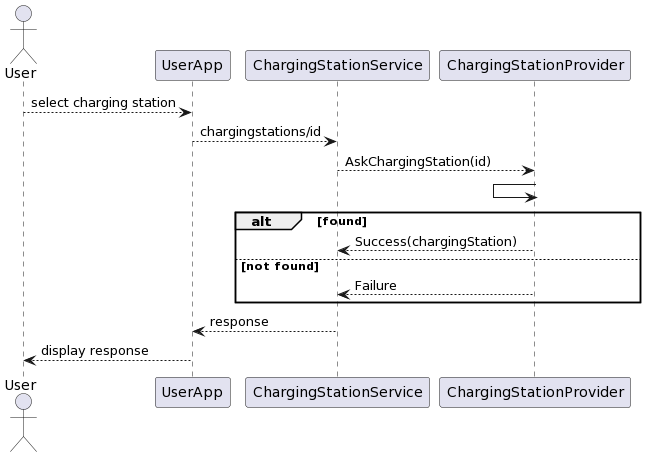
\includegraphics[width=\textwidth]{images/ask-station.png}
    \caption{Diagramma delle sequenze per la visualizzazione dello stato di una stazione di ricarica}
    \label{fig:ask-station}
\end{figure}

\paragraph{Visualizzazione dello stato di tutte le stazioni di ricarica all'interno della mappa}
L'utente interagisce con l'applicazione utente ("UserApp") e seleziona la visualizzazione della mappa.

L'applicazione utente invia quindi una richiesta per ottenere l'elenco di tutte le stazioni di ricarica disponibili al Charging Station Service. Il Servizio a sua volta comunica con il Provider.

Esso cerca tutte le stazioni di ricarica disponibili all'interno del suo registro. Successivamente, restituisce l'elenco completo delle stazioni di ricarica al Charging Station Service.

Quest'ultimo, a sua volta, restituisce l'elenco delle stazioni di ricarica all'applicazione utente. Infine, quest'ultima mostra le stazioni di ricarica all'interno della mappa all'utente.

Questa interazione è riassunta nel seguente diagramma di sequenza:

\begin{figure}[htbp]
    \centering
    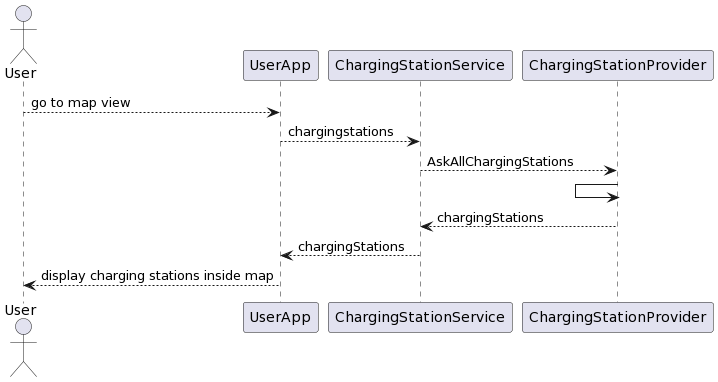
\includegraphics[width=\textwidth]{images/ask-all-stations.png}
    \caption{Diagramma delle sequenze per la visualizzazione dello stato di tutte le stazioni di ricarica all'interno della mappa}
    \label{fig:ask-all-stations}
\end{figure}

\paragraph{Prenotazione di una stazione di ricarica}
L'utente interagisce con l'applicazione utente e seleziona una stazione di ricarica da prenotare.

Successivamente, l'utente invia una richiesta di prenotazione al Charging Station Service tramite l'applicazione utente. Il Service comunica con il Charging Station Provider per richiedere la prenotazione della stazione selezionata.

Il Provider, a sua volta, comunica con il Charging Station Actor per effettuare la prenotazione. Se la stazione di ricarica è stata trovata, il Provider richiede all'attore della Stazione di Ricarica la prenotazione, il quale gli comunica l'esito.

Nel caso in cui la stazione di ricarica sia libera, l'attore della Stazione di Ricarica conferma la prenotazione e comunica al Provider che la prenotazione è avvenuta con successo. Il Provider, a sua volta, comunica al Service il successo della prenotazione, il quale comunica l'esito positivo all'applicazione utente.

Tuttavia, se la stazione di ricarica è già prenotata o è attualmente in uso per la ricarica, l'attore della Stazione di Ricarica comunica al Provider che la prenotazione non può essere effettuata. Il Provider comunica quindi al Service il fallimento della prenotazione, e questo a sua volta comunica all'applicazione utente l'esito negativo della prenotazione.

Nel caso in cui la stazione di ricarica non venga trovata, il Provider lo comunica al Service, che comunica quindi all'applicazione utente che la stazione di ricarica selezionata non è disponibile.\\

Questa interazione è riassunta nel seguente diagramma di sequenza:

\begin{figure}[htbp]
    \centering
    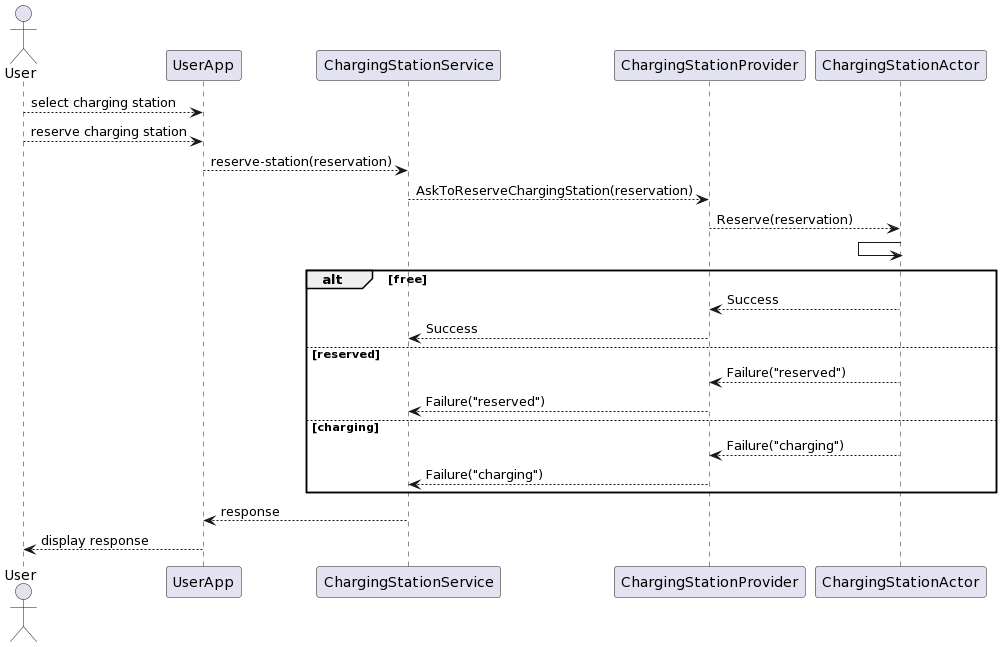
\includegraphics[width=\textwidth]{images/reserve-station.png}
    \caption{Diagramma delle sequenze per la prenotazione di una stazione di ricarica}
    \label{fig:reserve-station}
\end{figure}

\paragraph{Richiesta di ricarica di un veicolo}
L'utente interagisce con l'applicazione utente  e seleziona una stazione di ricarica. Successivamente, l'utente legge un codice QR associato alla stazione.

L'applicazione utente richiede quindi la possibilità di effettuare una ricarica presso la stazione selezionata e comunica al Charging Station Service la richiesta di ricarica. Il Servizio Stazioni di Ricarica comunica con il Charging Station Provider per richiedere l'autorizzazione alla ricarica.

Il Provider, a sua volta, comunica con il Charging Station Actor per autorizzare la ricarica.

Nel caso in cui la stazione di ricarica sia libera, l'attore comunica al Provider il successo della richiesta. Questo, a sua volta, comunica al Service il successo dell'autorizzazione, che lo comunica all'applicazione utente.

Se la stazione di ricarica è già prenotata, l'attore della Stazione di Ricarica verifica la prenotazione o lo stato di carica attuale. Se la prenotazione è valida, l'attore autorizza la ricarica. Altrimenti, se la prenotazione non è valida, l'attore comunica che la stazione non può essere utilizzata per la ricarica. Il Provider comunica quindi al Service il fallimento dell'autorizzazione, e questo a sua volta comunica all'applicazione utente l'esito negativo della richiesta di ricarica.

Se la stazione di ricarica è attualmente in uso, l'attore comunica che la stazione non può essere utilizzata per la ricarica. Il Provider comunica quindi al Service il fallimento dell'autorizzazione, e questo a sua volta comunica all'applicazione utente l'esito negativo della richiesta di ricarica.

Nel caso in cui la stazione di ricarica non venga trovata (caso "not found"), il Fornitore Stazioni di Ricarica comunica al Servizio Stazioni di Ricarica che la stazione non è stata trovata. Il Servizio Stazioni di Ricarica comunica quindi all'applicazione utente che la stazione di ricarica selezionata non è disponibile.

Questa interazione è riassunta nel seguente diagramma di sequenza:

\begin{figure}[htbp]
    \centering
    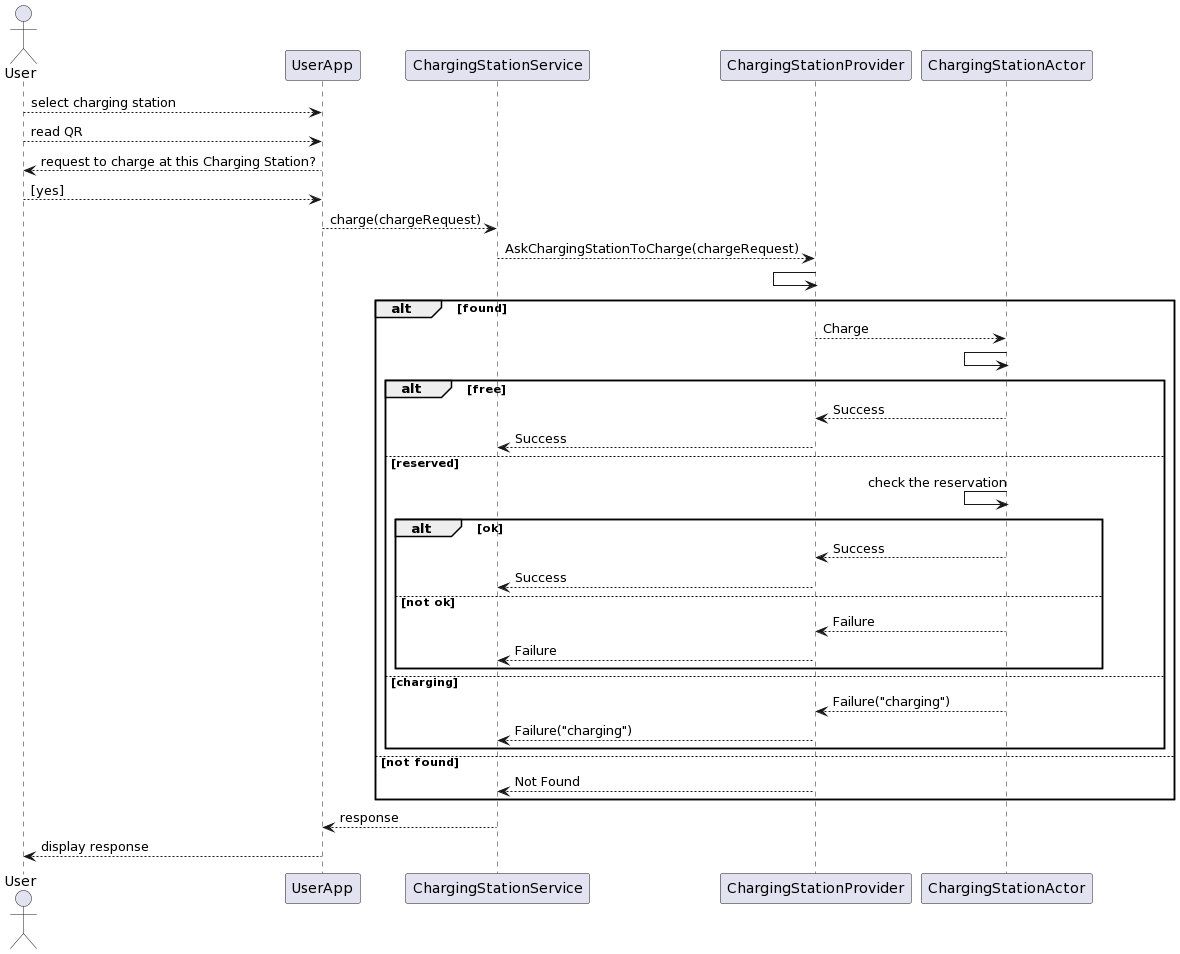
\includegraphics[width=\textwidth]{images/charge.png}
    \caption{Diagramma delle sequenze per la richiesta di ricarica di un veicolo}
    \label{fig:charge}
\end{figure}


\subsection{Design di Dettaglio}
%TODO: spiega le interazioni tra gli attori e componenti del sistema, con descrizione sia testuale che con diagrammi di sequenza.
La fase di Design di Dettaglio affronta la progettazione del sistema ad un livello di granularità più fine, siccome è in questa fase che ci si occupa di progettare i singoli componenti del sistema ed il loro protocollo di interazione.\\
\subsubsection{User Domain - A}
%TODO: spiegare le scelte di design principali della user app e dell'auth server con eventuali schemi

\subsubsection{Charging Station Domain}
Per quanto riguarda il dominio delle Charging Station, il gruppo ha deciso di utilizzare il paradigma ad \textbf{attori} per modellare il comportamento dei componenti del dominio e la
metodologia di interazione tra essi. \\

In questo paradigma, un attore è un'entità computazionale che può ricevere messaggi, elaborarli e rispondere con altri messaggi. Gli attori sono organizzati in gerarchie, dove ogni attore ha un solo attore padre e può avere più attori figli.\\
Ogni attore possiede una \textbf{mailbox}, ovvero una coda di messaggi in entrata, e un \textbf{behavior}, ovvero un insieme di regole che definiscono il comportamento dell'attore alla ricezione di un messaggio.\\

Una particolarità del modello ad attori è che può efficacemente modellare una macchina a stati finiti, in quanto l'attore può cambiare il suo comportamento in base al messaggio ricevuto e gli stati finiti corrispondono al set di messaggi ai quali l'attore può rispondere.\\
Questo ha permesso di modellare efficacemente il comportamento delle Charging Station, che possono trovarsi in uno dei seguenti stati:
\begin{itemize}
    \item \textbf{Free}: la stazione è disponibile per la ricarica.
    \item \textbf{Reserved}: la stazione è stata prenotata.
    \item \textbf{Charging}: la stazione è attualmente in uso per la ricarica.
\end{itemize}

La macchina a stati finiti per il Charging Station Actor è riassunta nel seguente diagramma:

\begin{figure}[htbp]
    \centering
    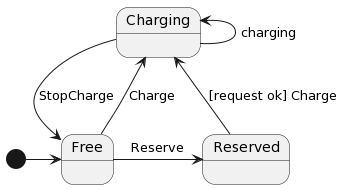
\includegraphics[width=\textwidth]{images/cs-state.png}
    \caption{Diagramma della macchina a stati finiti per il Charging Station Actor}
    \label{fig:cs-state}
\end{figure}


%Devono essere esposte le scelte progettuali operate nelle varie fasi di sviluppo dell'elaborato.\\

%In questa sezione devono essere documentati gli schemi di progetto relativamente all'architettura complessiva del sistema e alle sue componenti di rilievo che possano meritare un'analisi di dettaglio. Per le componenti software si può ricorrere ad esempio a diagrammi delle classi, di sequenza, stato, attività. Per le componenti hardware è possibile includere opportuni schemi in grado di descrivere l'architettura fisica adottata.\\

%Vincoli circa la lunghezza della sezione (escluse didascalie, tabelle, testo nelle immagini, schemi):

%\vspace{1cm}
%\begin{tabular}{l|rr}
% & Numero minimo di battute & Numero massimo di battute \\
% \hline
% 1 componente & 9000 & 18000 \\
% 2 componenti & 12000 & 21000 \\
% 3 componenti & 15000 & 24000 \\
% \hline
%\end{tabular}


\newpage